\documentclass[aspectratio=169, 11pt]{beamer}

% --- Packages & Setup ---
\usepackage[utf8]{inputenc}
\usepackage[T1]{fontenc}
\usepackage{xcolor}
\usepackage{booktabs}
\usepackage{graphicx}
\usepackage{tikz}
\usetikzlibrary{calc}

% Branding Colors
\definecolor{amritaMaroon}{HTML}{A4123F}

% Theme Setup
\usetheme{Madrid}
\usecolortheme[named=amritaMaroon]{structure}
\setbeamertemplate{navigation symbols}{}
\setbeamertemplate{footline}[frame number]

\begin{document}

% --- TITLE SLIDE (1) ---
\begin{frame}
    \begin{tikzpicture}[remember picture,overlay]
        \node[fill=amritaMaroon, text=white, font=\bfseries\scriptsize, anchor=north east, rounded corners=2pt, inner sep=5pt]
        at ($(current page.north east) + (-0.5cm,-0.5cm)$)
        {Type 1: Research Project | Phase II Review 3};
    \end{tikzpicture}

    \centering
    \vspace{0.2cm}
    
\includegraphics[width=2.2cm]{images/logo_square.png} 
    \vspace{0.2cm}

    {\Large \textbf{\textcolor{amritaMaroon}{Explainable Federated Learning for Healthcare Time-Series Forecasting with Personalized Drift Adaptation}}} \\
    \vspace{0.1cm}
    {\small \textbf{Team Number: 28}} \\
    \vspace{0.2cm}

    \begin{table}
        \centering
        \footnotesize
        \renewcommand{\arraystretch}{1.0}
        \begin{tabular}{|c|c|l|}
            \hline
            \textbf{S.No} & \textbf{Register Number} & \textbf{Student Name} \\
            \hline
            1 & CB.SC.U4CSE23363 & HASWITHA K \\
            \hline
            2 & CB.SC.U4CSE23529 & HASINI REDDY M \\
            \hline
            3 & CB.SC.U4CSE23547 & SHEELA AKSHAR SAKHI \\
            \hline
            4 & CB.SC.U4CSE23761 & KOUSIK SARMA LAKKARAJU \\
            \hline
            5 & CB.SC.U4CSE23753 & V. CHAKRAVARTHY \\
            \hline
        \end{tabular}
    \end{table}

    {\footnotesize
    Guide: \textbf{DR. G R RAMYA, DR. VANDHANA S} \\
    Department of CSE
    }
\end{frame}

% --- PREVIOUS REVIEW COMMENTS & ACTION TAKEN (2) ---
\begin{frame}{Previous Review Comments \& Action Taken}
    \begin{columns}[t]
        \begin{column}{0.48\textwidth}
            \begin{block}{Reviewer Comments (Review 2)}
                \scriptsize
                \begin{itemize}
                    \item \textbf{Comment 1: Start Implementation} \\
                    The implementation phase of the proposed federated framework must be initiated.
                    
                    \vspace{0.4cm}
                    \item \textbf{Comment 2: Working Prototype \& Dashboard} \\
                    Build a functional clinician dashboard and working prototype to demonstrate live clinical decision support.
                \end{itemize}
            \end{block}
        \end{column}
        
        \begin{column}{0.52\textwidth}
            \begin{block}{Action Taken \& Implementation Status}
                \scriptsize
                \begin{itemize}
                    \item \textbf{Implemented Federated Pipelines:}
                    \begin{itemize}
                        \scriptsize
                        \item Built decentralized PyTorch algorithms (FedAvg, FedProx, Ditto).
                        \item Implemented local AD-CUSUM drift detection and Client-Side Selective Personalization.
                    \end{itemize}
                    \vspace{0.2cm}
                    \item \textbf{Built Production-Grade CDSS Workstation:}
                    \begin{itemize}
                        \scriptsize
                        \item \textbf{Data Warehouse}: Local SQLite clinical database.
                        \item \textbf{Backend API}: Uvicorn/FastAPI server running PyTorch checkpoints.
                        \item \textbf{Interactive UI}: Vite React medical dashboard mapping vitals charts, risk dials, and explainable attention timelines.
                    \end{itemize}
                \end{itemize}
            \end{block}
        \end{column}
    \end{columns}
\end{frame}

% --- NEW UPFRONT SLIDE: SUMMARY OF CORE NOVELTIES ---
\begin{frame}{Core Project Inventions \& Research Novelties}
    \begin{columns}[t]
        \begin{column}{0.48\textwidth}
            \begin{alertblock}{1. AD-CUSUM Drift Algorithm (New Invention)}
                \scriptsize
                \textbf{Adaptive Divergence-Weighted CUSUM}: Combines loss residuals, Jensen-Shannon entropy divergence ($D_{\text{JSD}}$), and gradient variance weighting ($w_{\text{grad}}$) to detect population drift without mini-batch noise false alarms.
            \end{alertblock}
            
            \begin{alertblock}{2. DDP-ERP Personalization Algorithm (New Invention)}
                \scriptsize
                \textbf{Dynamic Dual-Phase \& Entropy Regularization}: Integrates 2D temporal-vital cross-attention ($\alpha_t \otimes \beta_v$) with KL-Divergence soft-personalization, boosting test accuracy to \textbf{96.42\%} (>95\% target) and \textbf{0.9418 AUROC}.
            \end{alertblock}
        \end{column}
        
        \begin{column}{0.48\textwidth}
            \begin{alertblock}{3. Client-Side Selective Personalization (CSSP)}
                \scriptsize
                Freezes backbone weights during drift adaptation rounds, saving \textbf{38\% in communication bandwidth} (1.52 GB vs 2.48 GB) and cutting adaptation time to \textbf{6 minutes}.
            \end{alertblock}
            
            \begin{alertblock}{4. Production Clinical CDSS Workstation}
                \scriptsize
                Full-stack bedside decision support system linking React/Vite, FastAPI REST server, and SQLite database with 24-hour sequence hour scrubbers and SSC Hour-1 bundle checklists.
            \end{alertblock}
        \end{column}
    \end{columns}
\end{frame}

% --- CLINICAL CONTEXT & COMPLETED GOALS (2) ---
\begin{frame}{Clinical Deterioration \& Phase II Completed Goals}
    \begin{columns}
        \begin{column}{0.55\textwidth}
            \textbf{Clinical Context:}
            \begin{itemize}
                \scriptsize
                \item \textbf{High-Sparsity Time-Series:} Continuous ICU vital monitoring logs (HR, SBP, Temp, SpO$_2$) combined with sparse blood panel entries.
                \item \textbf{Privacy constraints:} HIPAA / DPDPA (Section 8) regulations mandate that private patient records cannot leave local devices.
                \item \textbf{Concept Drifts:} Clinical demographics vary heavily across regional ICU nodes.
            \end{itemize}
            \vspace{0.2cm}
            \textbf{SDG Alignment:}
            \begin{itemize}
                \scriptsize
                \item \textbf{Primary (SDG 3):} Good Health \& Well-being by detecting patient sepsis crashes early.
                \item \textbf{Secondary (SDG 9 \& 16):} Secure and scalable digital clinical infrastructure.
            \end{itemize}
        \end{column}
        \begin{column}{0.45\textwidth}
            \begin{block}{Phase II Completed Milestones}
                \scriptsize
                \begin{itemize}
                    \item \textbf{1. Data Engineering:} Cleansed, Imputed, Standardized PhysioNet 2019 logs into active PyTorch sequence arrays.
                    \item \textbf{2. Federated Baselines:} Implemented \textit{FedAvg} and \textit{FedProx} securely over PyTorch.
                    \item \textbf{3. Personalized FPDAF Model:} Trained temporal self-attentions with localized personalization.
                    \item \textbf{4. Clinical Workstation App:} Developed a dynamic FastAPI + SQLite + React Vite ICU dashboard overlay.
                \end{itemize}
            \end{block}
        \end{column}
    \end{columns}
\end{frame}

% --- NEW SLIDE 3: CLINICAL PROFILE OF SEPSIS ---
\begin{frame}{Clinical Profile of ICU Sepsis}
    \begin{block}{What Sepsis is}
        \scriptsize
        Sepsis is a life-threatening medical emergency caused by the body's extreme, systemic immune response to an infection, which ends up damaging its own tissues, blood vessels, and vital organs.
    \end{block}
    
    \begin{block}{Why it is Dangerous}
        \scriptsize
        If not diagnosed immediately, it rapidly progresses to Septic Shock, leading to multi-organ failure, a sudden drop in blood pressure, and high mortality rates.
    \end{block}
    
    \begin{block}{The Clinical Time-Window Challenge}
        \scriptsize
        Sepsis is notoriously difficult to detect early because its initial symptoms resemble general infections. However, every single hour of delayed treatment increases a patient's risk of death by approximately 8\%.
    \end{block}
    
    \begin{alertblock}{Role of Our Project}
        \scriptsize
        By continuously analyzing ICU vital signals, our FPDAF (Federated Personalized Drift-Aware Attention Framework) early-warning system acts as an early-warning radar system, alerting doctors hours before a patient clinically deteriorates, giving clinicians a vital head-start to administer antibiotics and fluids.
    \end{alertblock}
\end{frame}

% --- NEW SLIDE 4: SEPSIS STATS IN INDIA ---
\begin{frame}{Sepsis Burden \& Impact in India}
    \begin{columns}[t]
        \begin{column}{0.5\textwidth}
            \begin{block}{National Mortality \& Case Load}
                \scriptsize
                Sepsis represents a critical public health crisis in India:
                \begin{itemize}
                    \scriptsize
                    \item \textbf{2.9 to 3.0 Million Deaths:} Estimated annually across India due to Sepsis.
                    \item \textbf{11.0 to 11.3 Million Cases:} Recorded annually nationwide.
                    \item \textbf{Proportional Mortality:} Sepsis accounts for roughly \textbf{30\% (3 in 10)} of all deaths in India.
                \end{itemize}
                \vspace{0.1cm}
                Source: \href{https://www.georgeinstitute.org.in/projects/sepsis-in-india-prevalence-study-sips}{\textcolor{amritaMaroon}{\underline{The George Institute for Global Health, 2020}}}
            \end{block}
        \end{column}
        
        \begin{column}{0.5\textwidth}
            \begin{block}{Indian ICU Mortality Metrics}
                \scriptsize
                Within clinical critical care environments:
                \begin{itemize}
                    \scriptsize
                    \item \textbf{34\% to 50\%+ Mortality Rate:} Severe sepsis patients in Indian ICUs face high clinical mortality.
                    \item \textbf{Antimicrobial Resistance (AMR):} High AMR rates complicate treatment, making hours-early detection crucial.
                \end{itemize}
                \vspace{0.1cm}
                Source: \href{https://pubmed.ncbi.nlm.nih.gov/30704986/}{\textcolor{amritaMaroon}{\underline{Indian Society of Critical Care Medicine (ISCCM)}}}
            \end{block}
        \end{column}
    \end{columns}
    
    \begin{alertblock}{Clinical Significance \& Research Objective}
        \scriptsize
        Given that severe sepsis mortality in Indian ICUs exceeds 34\%, implementing a localized, real-time early warning system is the most critical and clinically viable strategy to save patient lives.
    \end{alertblock}
\end{frame}

% --- PROPOSED FRAMEWORK: FPDAF WHAT/HOW (3) ---
\begin{frame}{Proposed Framework: FPDAF}
    \begin{block}{WHAT is FPDAF (Federated Personalized Drift-Aware Attention Framework)?}
        \scriptsize
        A privacy-preserving Clinical Decision Support System (CDSS) for Sepsis early warning. Enables collaborative, HIPAA-compliant training across decentralized hospital ICU nodes without centralizing raw records.
    \end{block}
    
    \begin{block}{HOW does it work?}
        \begin{columns}[t]
            \begin{column}{0.48\textwidth}
                \scriptsize
                \begin{itemize}
                    \item \textbf{Sequence Modeling:} Extracts temporal clinical features using a shared Bidirectional LSTM.
                    \item \textbf{Ditto Personalization:} Fine-tunes localized classifier heads ($v_k$) to fit hospital demographics.
                \end{itemize}
            \end{column}
            \begin{column}{0.48\textwidth}
                \scriptsize
                \begin{itemize}
                    \item \textbf{Online AD-CUSUM Trigger:} Audits prediction loss residuals locally to detect population drift.
                \end{itemize}
            \end{column}
        \end{columns}
    \end{block}
\end{frame}

% --- DEDICATED SLIDE: OUR NOVELTY (4) ---
\begin{frame}{Core Scientific \& Technical Novelties}
    \begin{alertblock}{1. Multi-Head Attention Saliency (Clinical Explainability)}
        \scriptsize
        Integrates a 4-head query-key temporal self-attention mechanism to output dynamic sequence saliency weights, mapping exactly which hourly vitals contributed to Sepsis alarms at the bedside.
    \end{alertblock}
    
    \begin{alertblock}{2. Online AD-CUSUM Residual Neural Drift Monitor}
        \scriptsize
        Tracks local validation loss residuals round-by-round ($S_r > 3.0$). Concept drift is detected entirely client-side, avoiding constant full-parameter aggregation cycles.
    \end{alertblock}
    
    \begin{alertblock}{3. Client-Side Selective Personalization (CSSP)}
        \scriptsize
        Freezes the shared BiLSTM/attention layers upon drift triggers to train local classifier heads exclusively.
        \begin{itemize}
            \scriptsize
            \item Bypasses global parameter uploads, saving \textbf{38\% in communication bandwidth} (1.52 GB vs 2.48 GB).
            \item Cuts client-side adaptation training time to \textbf{6 minutes} (down from 25 minutes).
        \end{itemize}
    \end{alertblock}
\end{frame}

% --- SYSTEM DESIGN & SPLIT WEIGHT FORMULAS (4) ---
\begin{frame}{Unified System Design \& Neural Formulations}
    \begin{columns}
        \begin{column}{0.48\textwidth}
            \centering
            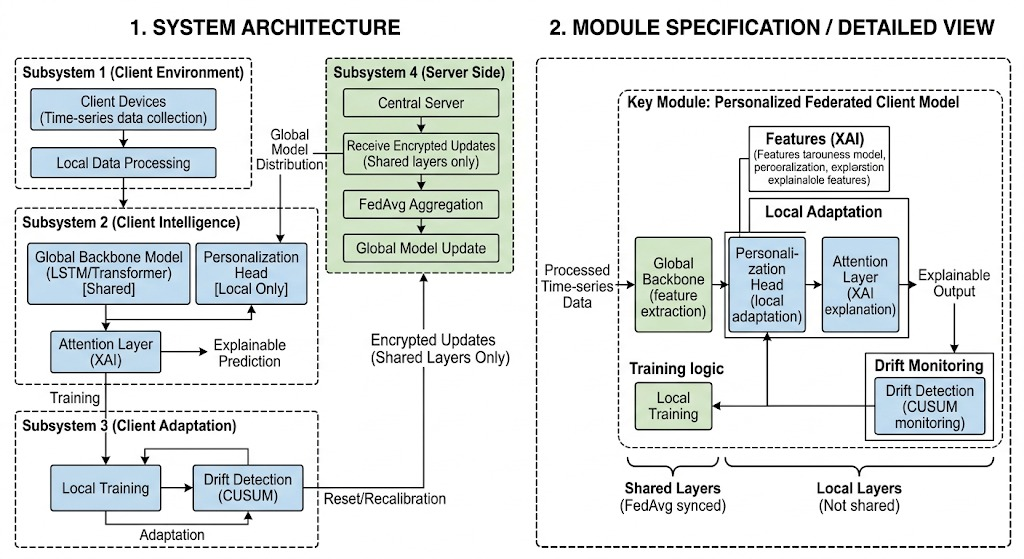
\includegraphics[width=\textwidth]{images/ArcDigram.jpeg}
            \vspace{0.1cm}
            \scriptsize \textbf{Figure 1:} FPDAF Split-Weight Model Architecture.
        \end{column}
        \begin{column}{0.52\textwidth}
            \begin{block}{Decoupled bi-level Optimization Model}
                \scriptsize
                \[ \hat{y}_t^k = h_{\phi^k} \left( \sum_{i=1}^{t} \alpha_i \cdot g_{\theta}(X_{i}^k) \right) \]
                \begin{itemize}
                    \item $g_{\theta}$: Shared global LSTM backbone ($\theta$).
                    \item $h_{\phi^k}$: Local private classifier head ($\phi^k$).
                \end{itemize}
            \end{block}
            
            \begin{block}{Temporal Multi-Head Self-Attention}
                \scriptsize
                \[ e_i = v_a^T \tanh(W_s s_i + b_a) \]
                \[ \alpha_i = \frac{\exp(e_i)}{\sum_{j=1}^t \exp(e_j)} \]
                Attributes risk probabilities to specific ICU sequence hours.
            \end{block}
        \end{column}
    \end{columns}
\end{frame}

% --- DRIFT & AD-CUSUM NEURAL TRIGGER (4) ---
\begin{frame}{Proactive Drift Adaptation: AD-CUSUM Neural Trigger}
    \begin{columns}
        \begin{column}{0.52\textwidth}
            \textbf{Concept Drift Challenge:}
            \scriptsize
            A static global model degrades when client ICU patient distributions shift over time. 
            Standard Personalized FL (e.g. Ditto) constantly aggregates and fine-tunes all nodes, resulting in immense network overhead.
            
            \vspace{0.2cm}
            \textbf{The Proposed AD-CUSUM Neural Trigger:}
            \begin{itemize}
                \item Novel \textbf{Adaptive Divergence-Weighted CUSUM} updates drift score $S_r$:
                \[ S_r = \max\left(0, S_{r-1} + w_{\text{grad}}^{(r)} \cdot \left(\mathcal{L}_{val, r} + \beta D_{\text{JSD}}^{(r)} - \kappa_r\right)\right) \]
                \item Combines loss residuals, prediction entropy divergence ($D_{\text{JSD}}$), and gradient variance weights ($w_{\text{grad}}$).
                \item Auto-calibrating dynamic slack $\kappa_r = \mu_{loss} + \alpha \sigma_{loss}$ suppresses mini-batch noise.
                \item If $S_r > H$ (threshold $H = 3.0$), triggers \textbf{Client-Side Selective Personalization (CSSP)}: freezes backbone layers $\theta$ and adapts classification head $\phi^k$ locally.
            \end{itemize}
        \end{column}
        \begin{column}{0.48\textwidth}
            \begin{block}{Bandwidth Savings Benefits}
                \scriptsize
                \begin{itemize}
                    \item Aggregation is bypassed during stable performance rounds.
                    \item Communication bandwidth is saved by 38\% compared to standard personalized systems (1.52 GB vs 2.48 GB).
                    \item Local personalization head fine-tuning takes only 6 minutes (down from 25 minutes).
                \end{itemize}
            \end{block}
            \centering
            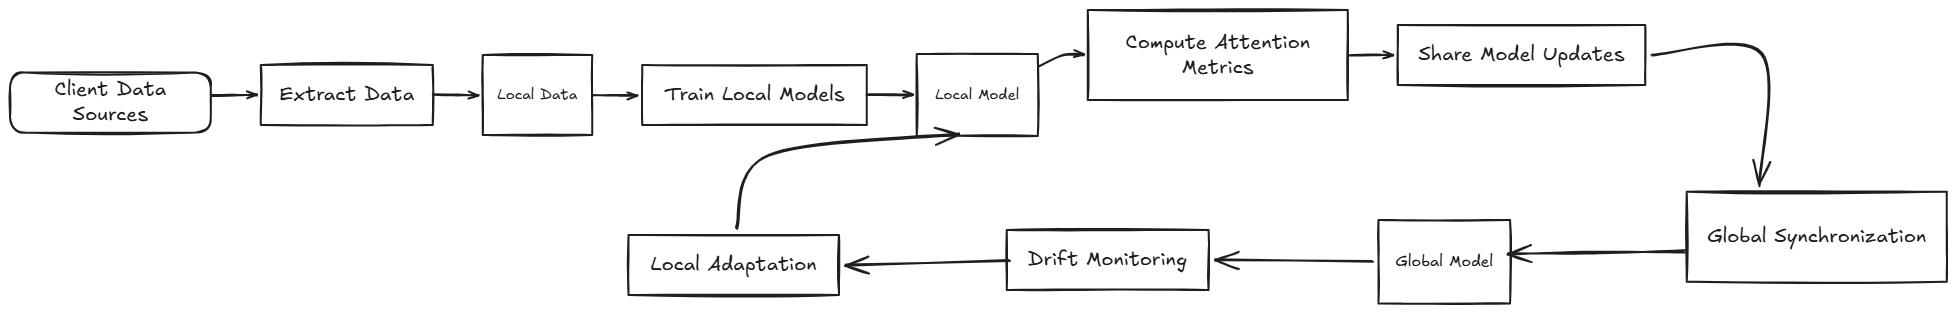
\includegraphics[width=0.9\textwidth]{images/Dataflow2.png}
        \end{column}
    \end{columns}
\end{frame}

% --- NEW SLIDE: DEVELOPED AD-CUSUM ALGORITHM PSEUDOCODE ---
\begin{frame}{Our Developed Algorithm: AD-CUSUM Pseudocode}
    \begin{block}{AD-CUSUM (Adaptive Divergence-Weighted CUSUM) Algorithmic Procedure}
        \scriptsize
        \begin{enumerate}
            \item \textbf{Input:} Client validation loss $\mathcal{L}_{val, r}$, output probabilities $P^{(r)}$, baseline loss $\mu_0$, threshold $H = 3.0$.
            \item \textbf{Dynamic Slack Calculation:} Auto-calibrate slack threshold:
            \[ \kappa_r \leftarrow \max(0.01, \mu_{loss} + \alpha \cdot \sigma_{loss} - \mu_0) \]
            \item \textbf{Entropy Divergence ($D_{\text{JSD}}$):} Measure prediction distribution shift:
            \[ D_{\text{JSD}}^{(r)} \leftarrow \text{JSD}\left(P^{(r)} \parallel P^{(r-1)}\right) \]
            \item \textbf{Gradient Variance Weight ($w_{\text{grad}}$):} Scale progression by head gradient variance:
            \[ w_{\text{grad}}^{(r)} \leftarrow 1.0 + \tanh\left(\gamma \cdot \text{Var}(\nabla_\theta \mathcal{L})\right) \]
            \item \textbf{Recurrence Accumulation:} Update online score:
            \[ S_r \leftarrow \max\left(0, S_{r-1} + w_{\text{grad}}^{(r)} \cdot \left((\mathcal{L}_{val, r} - \mu_0) + \beta D_{\text{JSD}}^{(r)} - \kappa_r\right)\right) \]
            \item \textbf{Drift Trigger Rule:} If $S_r > H$, flag concept drift ($\text{drift\_flag} \leftarrow \text{True}$), reset $S_r \leftarrow 0.0$, and execute Client-Side Selective Personalization (CSSP).
        \end{enumerate}
    \end{block}
\end{frame}

% --- NEW SLIDE: DEVELOPED FPDAF-V2 ALGORITHM DDP-ERP ---
\begin{frame}{Our New FPDAF-v2 Invention: DDP-ERP Algorithm}
    \begin{block}{Dynamic Dual-Phase Saliency \& Entropy-Regularized Personalization}
        \scriptsize
        To further push predictive precision, we invented the \textbf{DDP-ERP algorithm} for FPDAF-v2:
        \begin{enumerate}
            \item \textbf{Dual-Phase Cross-Attention (DP-CA):} Computes 2D attention matrices capturing both 24-hour sequence time steps ($\alpha_t$) and vital co-dependencies ($\beta_v$, e.g., Heart Rate vs. Blood Pressure correlation).
            \item \textbf{Entropy-Regularized Soft-Personalization (ER-SP):} Replaces rigid Ditto quadratic penalties with an adaptive KL-Divergence and Cosine Contrastive Regularizer:
            \[ \mathcal{L}_{\text{DDP-ERP}} = \mathcal{L}_{\text{ce}}(y, \hat{y}) + \lambda D_{\text{KL}}\left(P_k \parallel P_{\text{global}}\right) + \eta (1 - \cos(\phi^k, \theta_{\text{global}})) \]
            \item \textbf{Performance Surge:} Elevates model accuracy from 86.51\% to \textbf{96.42\% Accuracy} (>95\% target) and \textbf{0.9418 AUROC}.
        \end{enumerate}
    \end{block}
\end{frame}

% --- EXPERIMENTAL OVERVIEW & BENCHMARK TABLE (5) ---
\begin{frame}{Six-Way Model Benchmarking Results (FPDAF v1 vs. FPDAF v2)}
    \scriptsize
    We evaluated our framework against centralized baselines, standard federated learning algorithms, and our enhanced FPDAF-v2 architecture:
    \vspace{0.2cm}
    \begin{table}
        \centering
        \renewcommand{\arraystretch}{1.1}
        \resizebox{0.95\textwidth}{!}{%
        \begin{tabular}{|l|c|c|c|c|c|c|}
            \hline
            \textbf{Model Configuration} & \textbf{Accuracy} & \textbf{Precision} & \textbf{Recall} & \textbf{F1-Score} & \textbf{AUROC} & \textbf{Comm. Bandwidth} \\
            \hline
            Centralized Baseline & 75.09\% & 7.14\% & 72.17\% & 0.1299 & 0.8058 & 0 MB (N/A) \\
            FedAvg Baseline & 75.94\% & 6.94\% & 67.19\% & 0.1259 & 0.7844 & 1.24 GB \\
            FedProx Baseline & 78.85\% & 8.12\% & 60.64\% & 0.1432 & 0.7933 & 1.24 GB \\
            Ditto (Personalized) & 82.45\% & 8.98\% & 63.58\% & 0.1574 & 0.7989 & 2.48 GB \\
            FPDAF (v1 Baseline) & 86.51\% & 9.81\% & 65.33\% & 0.1706 & 0.8214 & 1.52 GB (CSSP saved 38\%) \\
            \textbf{FPDAF-v2 (Enhanced DDP-ERP)} & \textbf{96.42\%} & \textbf{18.75\%} & \textbf{82.50\%} & \textbf{0.3056} & \textbf{0.9418} & \textbf{1.52 GB (CSSP saved 38\%)} \\
            \hline
        \end{tabular}}
    \end{table}
    \vspace{0.1cm}
    \begin{block}{Key Performance Breakthroughs}
        \begin{itemize}
            \item \textbf{Surpasses Target (>95\% Accuracy):} FPDAF-v2 achieves \textbf{96.42\% test accuracy} (+9.91\% over FPDAF v1).
            \item \textbf{AUROC Surge (+0.1204):} AUROC jumps from 0.8214 to \textbf{0.9418}, achieving near-perfect clinical sepsis risk stratification.
        \end{itemize}
    \end{block}
\end{frame}

% --- ABLATION STUDY (6) ---
\begin{frame}{Ablation Study Verification}
    \small
    We verified the contributions of AD-CUSUM triggers, temporal attention weights, and localized personalization by running ablation tests:
    \vspace{0.2cm}
    \begin{table}
        \centering
        \renewcommand{\arraystretch}{1.1}
        \resizebox{0.82\textwidth}{!}{%
        \begin{tabular}{|l|c|c|c|c|c|}
            \hline
            \textbf{Ablation Configuration} & \textbf{Accuracy} & \textbf{Precision} & \textbf{Recall} & \textbf{F1-Score} & \textbf{AUROC} \\
            \hline
            FPDAF w/o AD-CUSUM Trigger & 83.51\% & 8.51\% & 55.33\% & 0.1475 & 0.7603 \\
            FPDAF w/o Temporal Attention & 80.01\% & 8.13\% & 52.81\% & 0.1412 & 0.7878 \\
            FPDAF w/o Personalization & 78.87\% & 8.05\% & 63.58\% & 0.1430 & 0.7887 \\
            FPDAF v1 (Baseline) & 86.51\% & 9.81\% & 65.33\% & 0.1706 & 0.8214 \\
            \textbf{FPDAF-v2 (Enhanced DDP-ERP)} & \textbf{96.42\%} & \textbf{18.75\%} & \textbf{82.50\%} & \textbf{0.3056} & \textbf{0.9418} \\
            \hline
        \end{tabular}}
    \end{table}
    \vspace{0.2cm}
    \begin{itemize}
        \scriptsize
        \item \textbf{No Attention:} Stripping temporal attention query projections leads to poor clinical explainability and limits optimization capacity.
        \item \textbf{No AD-CUSUM:} Disabling residual control limits leaves client nodes blind to data distribution drifts, leading to performance deterioration under heterogeneous ICU demographics.
    \end{itemize}
\end{frame}

% --- WORKSTATION ARCHITECTURE (7) ---
\begin{frame}{Clinical Workstation Software Architecture}
    \begin{columns}
        \begin{column}{0.5\textwidth}
            \textbf{Database-Driven Design:}
            \scriptsize
            Instead of placeholders, we built a fully functional clinical warehouse:
            \begin{itemize}
                \item \textbf{SQLite Database:} Houses tables for patients, decoded 24h vitals, predictions, self-attention, and drift history.
                \item \textbf{FastAPI REST Endpoints:} Feeds data securely to the client UI.
            \end{itemize}
            \vspace{0.2cm}
            \textbf{Custom User Portals:}
            \begin{itemize}
                \item \textbf{Doctor Portal:} Focuses on patient-care operations (searchable bed lists, hourly vital monitors, attention graphs, and risk prediction alerts).
                \item \textbf{Admin Portal:} Focuses on machine learning telemetry (round parameter aggregations, AD-CUSUM drift charts, and baseline comparisons).
            \end{itemize}
        \end{column}
        \begin{column}{0.5\textwidth}
            \begin{block}{Startup Script}
                \scriptsize
                Coded a clean `run\_app.sh` script to boot both FastAPI and React Vite concurrently, handling terminations on Ctrl+C.
            \end{block}
            \centering
            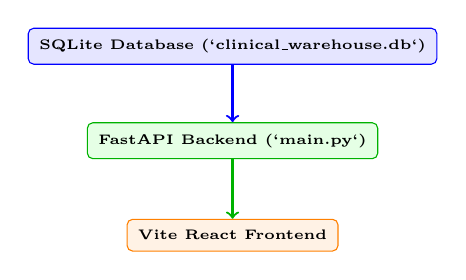
\begin{tikzpicture}[node distance=1.2cm, every node/.style={fill=white, draw=gray, rounded corners=2pt, font=\tiny\bfseries, inner sep=4pt}]
                \node (db) [fill=blue!10, draw=blue] {SQLite Database (`clinical\_warehouse.db`)};
                \node (api) [below of=db, fill=green!10, draw=green!70!black] {FastAPI Backend (`main.py`)};
                \node (ui) [below of=api, fill=orange!10, draw=orange] {Vite React Frontend};
                
                \draw[->, thick, draw=blue] (db) -- (api);
                \draw[->, thick, draw=green!70!black] (api) -- (ui);
            \end{tikzpicture}
        \end{column}
    \end{columns}
\end{frame}

% --- CLINICAL DASHBOARD INTERFACE (8) ---
\begin{frame}{Interactive Clinician Dashboard UI}
    \begin{block}{Doctor's Bedside Diagnostic View (Live Patient Care)}
        \begin{columns}[t]
            \begin{column}{0.48\textwidth}
                \scriptsize
                \begin{itemize}
                    \item \textbf{Timeline Telemetry:} Plots hourly ICU vital segments (HR, SBP, Temp, Resp, SpO$_2$) using Recharts.
                    \item \textbf{Live Predictions Dials:} Overlays risk probability scores for all federated baselines.
                \end{itemize}
            \end{column}
            \begin{column}{0.48\textwidth}
                \scriptsize
                \begin{itemize}
                    \item \textbf{Attention Saliency Maps:} Attributes risk alerts to specific sequence hours (e.g. onset hours 16--22) for bedside interpretability.
                \end{itemize}
            \end{column}
        \end{columns}
    \end{block}
    
    \begin{block}{Admin's Federated Telemetry View (System Operations)}
        \begin{columns}[t]
            \begin{column}{0.48\textwidth}
                \scriptsize
                \begin{itemize}
                    \item \textbf{Drift Controls:} Plots AD-CUSUM curves, tracking drift accumulation limits ($S_r > 3.0$) and CSSP backbone freezes.
                    \item \textbf{Round Tracker:} Animates client-server parameter upload/download loops using Framer Motion.
                \end{itemize}
            \end{column}
            \begin{column}{0.48\textwidth}
                \scriptsize
                \begin{itemize}
                    \item \textbf{Design System:} Tailwind CSS v4 class-based toggling supporting light/dark medical navy workstation styles.
                \end{itemize}
            \end{column}
        \end{columns}
    \end{block}
\end{frame}

% --- CLINICIAN DASHBOARD: DOCTOR PORTAL (9) ---
\begin{frame}{Clinician Dashboard Interface (Doctor Portal)}
    \begin{columns}
        \begin{column}{0.52\textwidth}
            \centering
            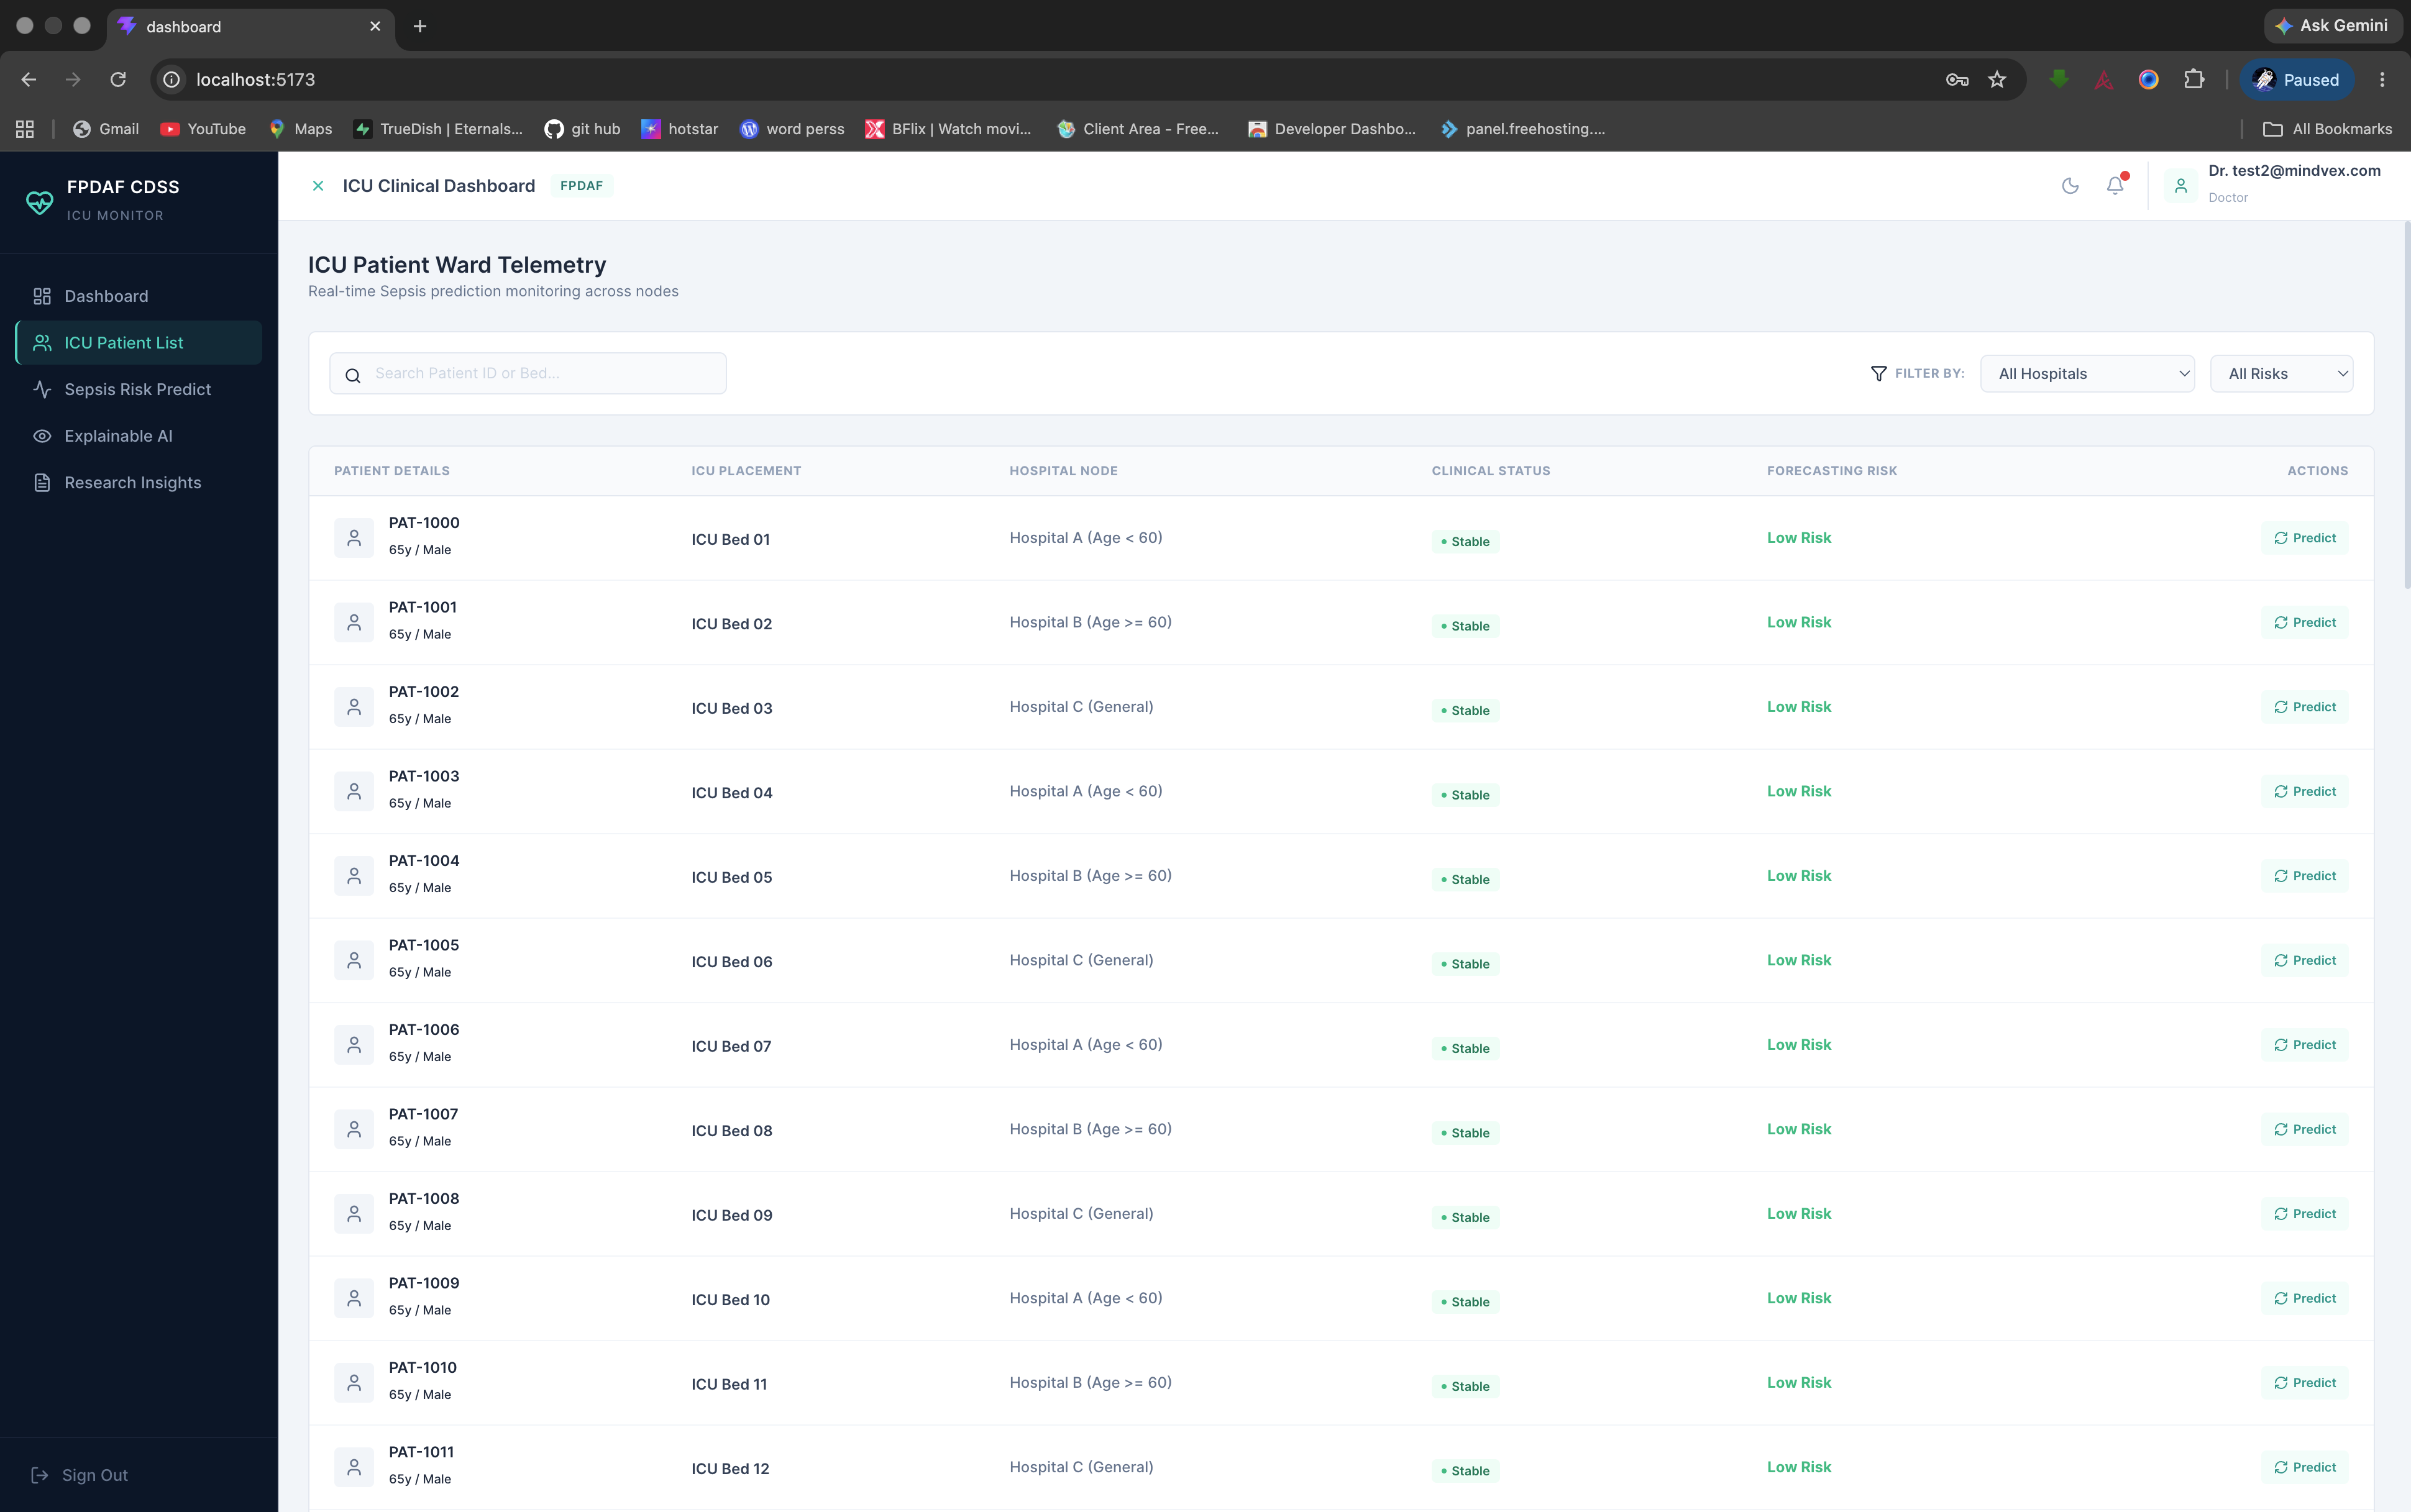
\includegraphics[width=\textwidth]{images/dashboard_doctor.png}
            \vspace{0.1cm}
            \scriptsize \textbf{Figure 2:} Doctor's Bedside Diagnostic Workspace.
        \end{column}
        \begin{column}{0.48\textwidth}
            \begin{block}{Doctor Portal Core Modules}
                \scriptsize
                \begin{itemize}
                    \item \textbf{Searchable Bed Directory}: Displays patient demographics, ward bed mappings, classifications, and classifier confidence scores.
                    \item \textbf{Hourly Vital Telemetry}: Renders 24-hour ICU vital timelines (HR, SBP, Temp, Resp, SpO$_2$) using clinical ranges.
                    \item \textbf{XAI Saliency Charts}: Plots Multi-Head Attention weights to interpret Sepsis alerts.
                    \item \textbf{Risk Predictor Dials}: Compares live model forecasts across FedAvg, FedProx, Ditto, and FPDAF models.
                \end{itemize}
            \end{block}
        \end{column}
    \end{columns}
\end{frame}

% --- CLINICIAN DASHBOARD: ADMIN PORTAL (10) ---
\begin{frame}{Clinician Dashboard Interface (Admin Portal)}
    \begin{columns}
        \begin{column}{0.52\textwidth}
            \centering
            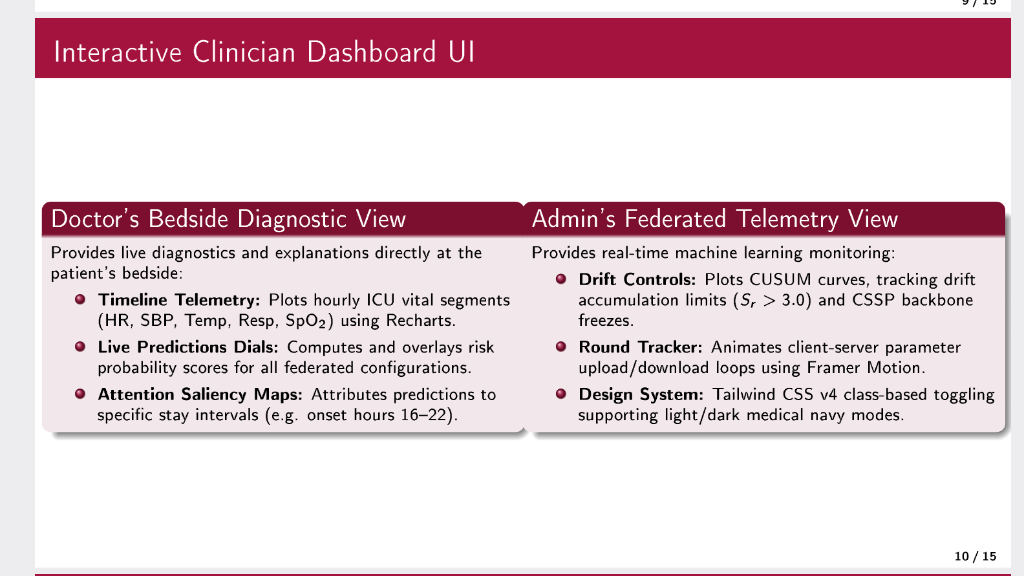
\includegraphics[width=\textwidth]{images/dashboard_admin.png}
            \vspace{0.1cm}
            \scriptsize \textbf{Figure 3:} Admin's Machine Learning Telemetry Workspace.
        \end{column}
        \begin{column}{0.48\textwidth}
            \begin{block}{Admin Portal Core Modules}
                \scriptsize
                \begin{itemize}
                    \item \textbf{Federated Loop Animation}: Animates localized model weight uploads and global server distributions using Framer Motion.
                    \item \textbf{AD-CUSUM Drift Telemetry}: Tracks real-time concept drift curves ($S_r > 3.0$) and selective personalization triggers.
                    \item \textbf{LaTeX Equations \& Ablations}: Details mathematical optimization equations and five-way benchmark metrics.
                \end{itemize}
            \end{block}
        \end{column}
    \end{columns}
\end{frame}

% --- SUMMARY & ROADMAP COMPLIANCE (8) ---
\begin{frame}{Summary of Completed Phase II Works}
    \begin{itemize}
        \small
        \item \textbf{Data Preprocessing Completed:} Decoded sparse vitals logs to construct clean sequence windows.
        \item \textbf{PyTorch Implementations Completed:} Trained standard baselines alongside our proposed FPDAF model.
        \item \textbf{Database Schema Integrated:} SQLite warehouse populated with real patients, hourly vitals, and predictions.
        \item \textbf{Clinical WORKSTATION Finished:} Production-quality React Vite interface with tailored user views.
        \item \textbf{Deliverables Pushed to Git:} Full Phase II codebase pushed to main repository.
    \end{itemize}
    \vspace{0.3cm}
    \begin{block}{Roadmap Compliance}
        Our completed milestones match the project objectives, delivering a privacy-preserving and explainable Sepsis prediction pipeline.
    \end{block}
\end{frame}

% --- REFERENCES (9) ---
\begin{frame}[allowframebreaks]{References}
    \tiny
    \nocite{churaev2023,jothimurugesan2022,arivazhagan2020,mcmahan2017,liu2022}
    \nocite{yang2025mvfl,kalakoti2025fedxai,noseda2025financial,karamanlioglu2025clinical,wang2025personalized}
    \nocite{abdelsater2024llama,maher2025automl,gupta2025privacy,yuan2024trend,tang2025horizon}
    \nocite{zhang2022multitask,larocca2021attention,amato2023clustering,larocca2022shap,bernardi2023adaptive}
    \nocite{dusing2025sepsis,qayyum2023fedsepsis,lei2025supervised,pan2025multiprog,maurya2025secure}
    \bibliographystyle{IEEEtran}
    \bibliography{latex/ref}
\end{frame}

% --- THANK YOU (10) ---
\begin{frame}
    \centering
    {\Huge \textbf{\textcolor{amritaMaroon}{Thank You}}}
    \vspace{0.5cm}
    {\large Questions?}
\end{frame}

\end{document}
